\documentclass[12pt,a4]{article}







\usepackage{graphicx,amsmath,amssymb,amsthm, boxedminipage,xcolor}

%\usepackage[lined,boxed]{algorithm2e}

\usepackage{algorithm}
\usepackage{algpseudocode}

%\usepackage{algorithmic}
\usepackage{algpseudocode}
\usepackage{amsmath}
\usepackage{graphics}
\usepackage{epsfig}

\newtheorem{theorem}{Theorem}[section]
\newtheorem{proposition}[theorem]{Proposition}
\newtheorem{lemma}[theorem]{Lemma}
\newtheorem{corollary}[theorem]{Corollary}
\newtheorem{definition}[theorem]{Definition}

\newtheorem*{theorem*}{Theorem}
\newtheorem*{lemma*}{Lemma}
\newtheorem*{proposition*}{Proposition}


\newtheorem{exercise}[theorem]{Exercise}
\newtheorem{exerciseD}[theorem]{*Exercise}
\newtheorem{exerciseDD}[theorem]{**Exercise}

\let\oldexercise\exercise
\renewcommand{\exercise}{\oldexercise\normalfont}

%\let\oldexerciseD\exerciseD
%\renewcommand{\exerciseD}{\oldexerciseD\normalfont}

%\let\oldexerciseDD\exerciseDD
%\renewcommand{\exerciseDD}{\oldexerciseDD\normalfont}

\newcommand{\E}{\mathbb{E}}
%\newcommand{\nth}[1]{#1^{\textsuperscript{th}}}
\newcommand{\scalar}[2]{\ensuremath{\langle #1, #2\rangle}}
\newcommand{\floor}[1]{\left\lfloor #1 \right\rfloor}
\newcommand{\ceil}[1]{\left\lceil #1 \right\rceil}
\newcommand{\norm}[1]{\|#1\|}
\newcommand{\pfrac}[2]{\left(\frac{#1}{#2}\right)}
\newcommand{\nth}[1]{#1^{\textsuperscript{th}}}
\newcommand{\core}{\textnormal{core}}



\newif\ifsolution

\solutionfalse

\newcommand{\answer}[1]{
\ifsolution
{\color{blue} #1}
\else
\fi
}



\newcommand{\poly}{\textnormal{poly}}
\newcommand{\quasipol}{\textnormal{quasipol}}
\newcommand{\ssubexp}{\textnormal{stronglySubExp}}
\newcommand{\wsubexp}{\textnormal{weaklySubExp}}
\newcommand{\simplyexp}{\textnormal{E}}
\newcommand{\expo}{\textnormal{Exp}}



\newcommand{\N}{\mathbb{N}}
\newcommand{\nn}{\mathbb{N}_0^n}
\newcommand{\R}{\mathbb{R}}
\newcommand{\Z}{\mathbb{Z}}


\definecolor{darkgreen}{rgb}{0,0.6,0}


\date{}

\title{
  Mathematical Foundations \\of \\Computer Science\\
  \vspace{3mm}
{\normalsize CS 499,	Shanghai Jiaotong University,  Dominik Scheder}
}

\begin{document}

\maketitle

%\begin{quotation}
%  You are welcome to discuss the exercises in the discussion
%  forum. Please take them serious. Doing the exercises is as important
%  than watching the videos.
%
%  I intentionally included very challenging exercises and marked them
%  with one or two ``$*$''. No star means you should be able to solve
%  the exercises without big problems once you have understood
%  the material from the video lecture. One star means it requires 
%  significant additional thinking. Two stars means it is not 
%  unlikely that you will fail to solve them, even once you have understood
%  the material and thought a lot about the exercise. Don't feel bad
%  if you fail. Failure is part of learning.
%
%  This is the first time this course is online. Thus there might be mistakes
%  (typos or more serious conceptual mistakes) in the exercises. I will be 
%  grateful if you point them out to me!
%\end{quotation}




\setcounter{section}{2}


\begin{itemize}
 \item Homework assignment published on Tuesday, 2018-03-13
 \item Submit questions and first solutions by Sunday, 2018-03-18, 12:00 by email to dominik.scheder@gmail.com  and the TAs.
 \item You will receive feedback by Wednesday, 2018-03-21
 \item Revise your solution and submit your final solution by Sunday, 2018-03-25 by  email to dominik.scheder@gmail.com and the TAs.
\end{itemize}



\section{Basic Counting}

A function $[m] \rightarrow [n]$ is {\em monotone} if $f(1) \leq f(2) \leq \dots \leq f(m)$.
It is  {\em strictly monotone} if $f(1) < f(2) < \dots < f(m)$.

\begin{exercise}
   Find and justify a closed formula for the number of strictly
   monotone functions from $[m]$ to $[n]$.
\end{exercise}
\textbf{Solution.}
    We choose $m$ elements in $[n]$, and match each one with the element in $[n]$ with the same order. Note that if $n < m$, there is no feasible matching like that, and the solution is $0$.
$$
    N_{m,n}=\binom{n}{m}
$$

\begin{exercise}
   Find and justify a closed formula for the number of monotone functions from $[m]$ to $[n]$.
\end{exercise}
\textbf{Solution.}
    We choose $1$ to $m$ elements in $[n]$, and then we need to allocate elements in $[m]$ to them. If we choose $i$ elements in $[n]$, $[m]$ needs to be divided into $i$ parts. Note that elements in each part is continuous in order, so we can insert $i-1$ plates into intervals of $[m]$, where there are $m-1$ intervals. Then we can use the formula $\binom{n}{m}=\binom{n}{n-m}$. At last we can use a combinatorial interpretation to get the final formula for the number of monotone functions from $[m]$ to $[n]$.
$$
    N_{m,n}=\sum^m_{i=0}(\binom{n}{i}\times\binom{m-1}{i-1})=\sum^m_{i=1}(\binom{n}{i}\times\binom{m-1}{m-i})=\binom{m+n-1}{m}
$$

\textbf{Remark.} By ``closed'' I mean something using expressions like $\times$, $+$,
${n \choose k}$, $n!$, but not $\sum$ or $\prod$.
For example, ${n \choose k^2}$ is a closed formula but
$\sum_{k=0}^n {n \choose k}$ is not.


\begin{exercise}
  Prove that $\sum_{k=0}^n {n \choose k}^2 = {2n \choose n}$ for every $n \geq 0$ by finding a combinatorial interpretation.
\end{exercise}
\textbf{Solution.}
    Obviously $\sum_{k=0}^n {n \choose k}^2 = \sum_{k=0}^n {n \choose k}\times{n \choose {n-k}}$. Assume there are two sets each of which has $n$ elements, and we need to choose $n$ elements from them. One way is to choose $k$ ($0\leq k\leq n$) elements from one set and then choose $n-k$ elements from the other, which is $\sum_{k=0}^n {n \choose k}^2$. Another way is to see them as a whole which has $2n$ elements, and then we choose $n$ elements from it, which is ${2n \choose n}$.
\begin{exercise}[From the textbook]
   Find a closed formula for $\sum_{k=m}^n {k \choose m}{n \choose k}$ and prove it combinatorially, i.e., by giving an
   interpretation.
\end{exercise}

\begin{exercise}
   Let $B_n$ be the number of partitions of the set $[n]$ (this is the same as the number
   of equivalence relations on $[n]$). This is called the Bell number, thus we
   denote it $B_n$.
   Prove that the following recursive formula
   for $B_n$ is correct:
   \begin{align*}
     B_0 & = 1 \\
     B_{n+1} & = \sum_{k=0}^n {n \choose k} B_k  \ .
   \end{align*}
\end{exercise}

\begin{exercise}
  Let $P_n$ be the number of ways to write the natural number $n$ as a sum $
  a_1 + a_2 + \cdots + a_k$ such that
  $1 \leq a_1 \leq a_2 \leq \dots \leq a_k$. For example, $3$ can be written
  as $3$, $2 + 1$, and $1 + 1 + 1$, so $P_3 = 3$.
   Find a recursive formula for $P_n$.\\

   \textbf{Remark.} The formula might not be as simple as the above for $B_n$. Be creative!
   Start by writing a simple recursive program that computes $P_n$.
\end{exercise}

\textbf{Solution.}
    Note $Q_n(i)$ to be the number of ways to write the natural number $n$ as a sum $
  a_1 + a_2 + \cdots + a_k$ such that
  $1 \leq a_1 \leq a_2 \leq \dots \leq a_k$ and $a_1 = i$.
\par Obviously, the number of different ways to write $n$ equals to the sum of number of different ways where $a_i=1,2,...,n$. We have
\begin{equation}
P_n = \sum_{i=1}^n Q_n(i) 
\end{equation}
\par For convenience, we let $Q_n(i) = 0$ if $i>n$.
\par Now we try to find a recursive formula for $Q_n(i)$, after that we can get the formula for $P_n$ using the equation above. 
\par We can view the number of ways to write natural number $n$ as the number of ways to put boards to segment a string of balls so that the number of balls located in th left side is less or equal to number of balls located in the right side. We observe that
\begin{equation}
Q_n(i) = \sum_{j=i}^{n-i} Q_{n-i}(j)
\end{equation}
The equation has the following explanation. We start by segmenting $i$ balls out of $n$ balls in the left side, then there are $n-i$ balls remaining in the right side. If we continue to segment the remaining balls, we can start by segment $j$ balls and $i \leq j$. So the total number of ways to segment $n$ balls. 

\newpage
\begin{figure}[hpbt]
\begin{center}
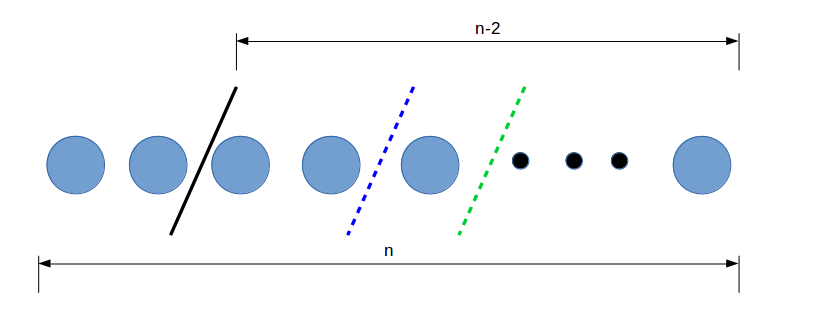
\includegraphics[width = 0.8 \textwidth]{ball3_6.png}
\end{center}
\end{figure}
\par As the picture shows, we want to get the formula for $Q_n(2)$. We first segment two balls in the left and there are $n-2$ balls remaining. Then we may start by any number $j \ge 2$. Then the total number of ways to segment balls is $\sum_{j=2}^{n-2} Q_{n-2}(j)$.

\par Now we get the recursive formula for $Q_n(i)$ and thus get formula for $P_n$.
\begin{equation}
\begin{aligned}
Q_1(1) &= 1 \\
Q_n(i) &= \sum_{j=i}^{n-i} Q_{n-i}(j) \\
P_n &= \sum_{i=1}^n Q_n(i) 
\end{aligned}
\end{equation}


\end{document}

